% Created 2020-11-05 Thu 14:05
% Intended LaTeX compiler: pdflatex
\documentclass{article}
       \usepackage[T1, T2A]{fontenc}
\usepackage[lutf8]{luainputenc}
\usepackage[russian, english]{babel}
\usepackage{minted}
\usepackage{graphicx}
\usepackage{longtable}
\usepackage{hyperref}
\usepackage{natbib}
\usepackage{amssymb}
\usepackage{amsmath}
\usepackage{grffile}
\usepackage{wrapfig}
\usepackage{rotating}
\usepackage{placeins}
\usepackage[normalem]{ulem}
\usepackage{amsmath}
\usepackage{textcomp}
\usepackage{tikz}
\usepackage{capt-of}
       
       \usepackage{geometry}
       \geometry{a4paper,left=2.5cm,top=2cm,right=2.5cm,bottom=2cm,marginparsep=7pt, marginparwidth=.6in}
\author{Ilya Yaroshevskiy}
\date{\today}
\title{Testing org to pdf}
\hypersetup{
 pdfauthor={Ilya Yaroshevskiy},
 pdftitle={Testing org to pdf},
 pdfkeywords={},
 pdfsubject={},
 pdfcreator={Emacs 27.1 (Org mode 9.3)}, 
 pdflang={English}}
\begin{document}

\maketitle
\tableofcontents


\section{Test org to pdf}
\label{sec:orgac345b3}
\subsection{Code blocks}
\label{sec:org89144ae}

\begin{minted}[frame=lines,linenos=true,mathescape]{haskell}
main = putStrLn "Hello World!"
\end{minted}

\begin{minted}[frame=lines,linenos=true,mathescape]{c}
#include <stdio.h>

int main() {
    printf("Hello World!")
    return 0;
}
\end{minted}

\begin{minted}[frame=lines,linenos=true,mathescape]{python}
print("Hello World!")
\end{minted}

\begin{minted}[frame=lines,linenos=true,mathescape]{bash}
echo "Hello World!"
\end{minted}

\begin{minted}[frame=lines,linenos=true,mathescape]{clojure}
(print "Hello World!")
\end{minted}


\begin{listing}[htbp]
\begin{minted}[frame=lines,linenos=true,mathescape]{c++}
#include <iostream>

int main() {
    std::cout << "Hello Wordl!" << std::endl;      (sc)
    return 0;
}
\end{minted}
\caption{C++ Hello world}
\end{listing}

Tes reference sc

\begin{minted}[frame=lines,linenos=true,mathescape]{python}
return "Test"
\end{minted}

\begin{minted}[frame=lines,linenos=true,mathescape]{python}
return "Wow it's: {}".format(s)
\end{minted}

\subsection{Graphs}
\label{sec:org99e9464}

\begin{figure}[H]
\centering
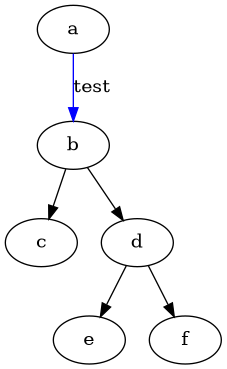
\includegraphics[scale=0.5]{TMP.png}
\caption{Test1}
\end{figure}

\begin{figure}[H]
\centering
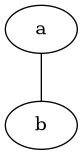
\includegraphics[scale=0.5]{TMP2.png}
\caption{Test 2}
\end{figure}

\begin{aligned}
\[e^{i \pi} = 1\]
\end{aligned}


And now \textbf{Русские вперед}
\subsection{Plots}
\label{sec:org1f1fdee}

\begin{center}
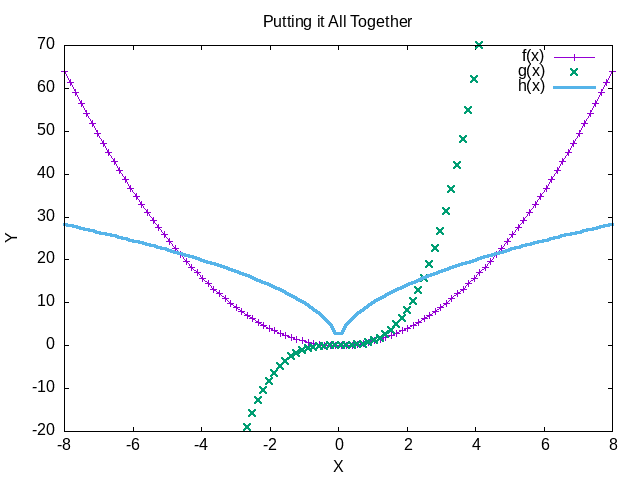
\includegraphics[width=.9\linewidth]{plot1.png}
\end{center}


\begin{minted}[frame=lines,linenos=true,mathescape]{python}
import math
import numpy as np
y = lambda x: x**2
X = list(np.arange(-10, 10, 0.25))
Y = []
for x in X:
    Y += [y(x)]
return list(zip(X, Y))
\end{minted}

\begin{center}
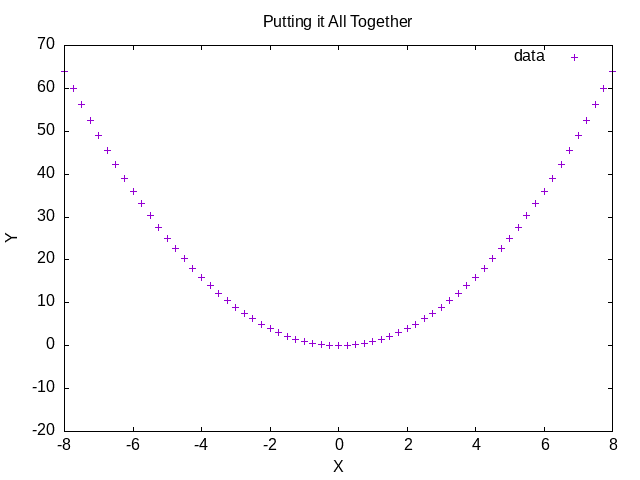
\includegraphics[width=.9\linewidth]{plot2.png}
\end{center}

\begin{minted}[frame=lines,linenos=true,mathescape]{python}
return data[1]
\end{minted}


\begin{center}
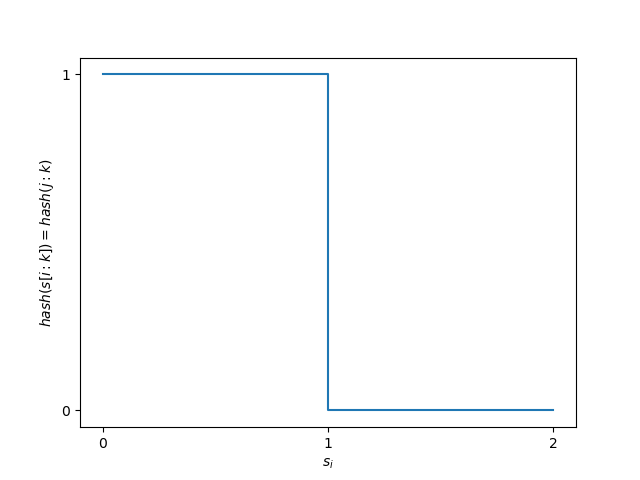
\includegraphics[width=.9\linewidth]{13_2.png}
\end{center}
\subsection{Tikz}
\label{sec:org3b99ac8}
\begin{tikzpicture}
\draw[gray, thick] (-1,2) -- (2,-4);
\draw[gray, thick] (-1,-1) -- (2,2);
\filldraw[black] (0,0) circle (2pt) node[anchor=west] {Intersection point};

\end{tikzpicture}
\end{document}
